\chapter{基于知识蒸馏的模型学习}[Distilling Knowledge for Search-based Structured Prediction]\label{chp:distill}

\section{简介}[Introduction]

基于搜索的结构预测将自然语言结构(如词性序列,句法树,翻译,语义图等)
的生成过程建模为一个搜索问题\cite{collins-roark:2004:ACL,
	liang-EtAl:2006:COLACL,
	zhang-clark:2008:EMNLP,
	huang-fayong-guo:2012:NAACL-HLT,
	NIPS2014_5346,
	goodman-vlachos-naradowsky:2016:P16-1}。
由于较高的准确率与较快的运行速度,
基于搜索的结构预测近年来获得了很多关注。
基于搜索的结构预测依靠一个概率化的策略函数
来指导搜索过程。
这个策略函数通常通过模仿\textit{参考策略}进行学习。
这种模仿的过程通常包括训练一个分类器,
使其能够在
参考策略遇到的状态上预测出参考策略的搜索动作。
这种模仿方式有时候是有问题的。
其中一个问题是参考策略是有歧义的,
即不同的搜索动作都可以达到正确的结构。
但在模仿过程中,
只有一种动作被用作正确实例来训练分类器\cite{goldberg-nivre:2012:PAPERS}。
另一个问题是训练测试不一致的问题,
即训练过程是在正确的搜索状态中完成的,
但在测试过程中,
学到的策略可能会进入不正确的搜索状态\cite{pmlr-v9-ross10a,pmlr-v15-ross11a}。
这些问题都影响了基于搜索的结构预测的泛化性以及性能。
%In practice,
%the reference policy can sometimes be sub-optimal because of
%the ambiguities in the data and doesn't generalize well
%where discrepancy exists between training and testing.

\begin{figure}[t]
	\tikzstyle{ann} = [above, text width=5em, text centered]
	\tikzstyle{data} = [draw, minimum width=3em, fill=red!20, minimum height=1.5em, text centered, text width=4.5em, rounded corners, drop shadow]
	\tikzstyle{model}=[draw, fill=white!20, minimum width=4.5em, minimum height=1.5em, text width=4.5em, text centered, drop shadow]
	\centering
	\begin{tikzpicture}
	\node (data) [data]  {Training data};
	\path (data.west)+(-1.5,0) node (refp)[model] {Reference policy};
	\path (data.east)+(1.5,0) node (expp)[model] {Exploration policy};
	\path (refp.north)+(0,1) node (refs)[data] {Reference states};
	\path (refs.north)+(0,1) node (reft)[data] {NLL\\loss};
	\path (expp.north)+(0,1) node (exps)[data] {Exploration states};
	\path (exps.north)+(0,1) node (expt)[data] {Distillation loss};
	\path (expt.west)+(-1.5,0) node (distill)[model] {Distilled model};
	\path (refp.south)+(0,-1.5) node (m1)[model] {model$_1$};
	\path (data.south)+(0,-1.2) node (ens)[above, text width=10em, text centered] {Ensemble model}; 
	\path (data.south)+(0,-1.7) node (dots)[ann] {$\dots$};
	\path (expp.south)+(0,-1.5) node (mm)[model] {model$_M$};
	
	\path (refp.south)+(0,-0.7) node (ens14) {};
	\path (expp.south)+(0,-0.7) node (ens34) {};
	\path (refs.south)+(-0.5,0.1) node (refssouth14) {};
	\path (refs.south)+(+0.5,0.1) node (refssouth34) {};
	\path (reft.south)+(-0.5,0.1) node (reftsouth14) {};
	\path (reft.south)+(+0.5,0.1) node (reftsouth34) {};
	
	\draw[->, thick] (data.west) to (refp.east);
	\draw[->] (refp.north)+(-0.5,0) to (refssouth14);
	\draw[->] (refs.north)+(-0.5,0) to (reftsouth14);
	\draw[->] (reft.west) to [bend right=13] (m1.west);
	
	\draw[->, color=red, dashed, thick] (refp.north)+(+0.5,0) to (refssouth34);
	\draw[->, color=red, dashed, thick] (refs.north)+(+0.5,0) to (expt.south);
	\draw[->, color=red, dashed, thick] (ens14) to (refp.south);
	
	\draw [->, color=blue, thick] (data.east) to (expp.west);
	\draw [->, color=blue, thick] (expp.north) to (exps.south);
	\draw [->, color=blue, thick] (exps.north) to (expt.south);
	\draw [->, color=blue, thick] (expt.west) to (distill.east);
	\draw [->, color=blue, thick] (ens34) to (expp.south);
	
	\path (m1.west |- m1.south)+(-0.2,-0.2) node (a) {};
	\path (mm.east |- mm.south)+(+0.2,-0.2) node (b) {};
	\path (ens.north -| mm.east)+(+0.2,+0.1) node (c) {};
	\path (m1.west |- ens.north)+(-0.2,+0.1) node (d) {};
	\path[rounded corners, draw=black, dashed] (a) rectangle (c);
	\end{tikzpicture}
	\caption{Workflow of our knowledge distillation for search-based
		structured prediction. The yellow bracket represents the ensemble
		of multiple models trained with different initialization. 
		The dashed red line shows our {\it distillation from reference} (\S\ref{sec:distill_ref}).
		The solid blue line shows our {\it distillation from exploration} (\S\ref{sec:distill_explore}).}\label{fig:distill:workflow}
\end{figure}

前人工作从两个方面解决这一问题。
为了解决训练数据的歧义问题,
文献\inlinecite{Dietterich2000}使用\textit{集成学习}。
为了解决训练测试不一致的问题,
前人工作\cite{
	pmlr-v9-ross10a,
	pmlr-v15-ross11a,
	goldberg-nivre:2012:PAPERS,
	NIPS2015_5956,
	goodman-vlachos-naradowsky:2016:P16-1}在训练过程中鼓励模型探索错误的状态。
本文提出使用\textit{知识蒸馏}\cite{DBLP:journals/corr/HintonVD15}的手段统一地解决这两类问题。
本文提出从一个由不同初始化的模型进行集成获得的复杂模型中蒸馏出一个简单模型。
蒸馏的过程可以描述为用简单模型在参考策略的状态上匹配复杂模型的概率输出。
除此之外,本文也在学习过程中允许集成模型探索搜索空间,
并在探索到的状态中学习模型。
将这两种蒸馏过程进行结合可以进一步提高模型的性能。
本文提出的模型的流程图如图\ref{fig:distill:workflow}所示。

本文在两个典型的基于搜索的结构预测问题 --- 基于转移的依存句法分析
以及神经网络机器翻译上进行了实验。
两项实验的结果均超过了强基线系统的结果,
这显示了本文提出方法的有效性。
在依存句法分析的实验中,相对基线系统的提升是1.32;
在机器翻译实验中,相对基线系统的提升是2.65。
机器翻译的实验性能也超出了前人基于贪心搜索的最好结果。

本文的主要贡献如下:
\begin{itemize}
	\item We study the knowledge distillation in search-based structured prediction
	and propose to distill the knowledge of an ensemble into a single model by
	learning to match its distribution on both the reference states (\S\ref{sec:distill_ref}) and exploration
	states encountered when using the ensemble to explore the search space (\S\ref{sec:distill_explore}).
	A further combination of these two methods is also proposed to improve the
	performance (\S\ref{sec:distill_both}).
	
	\item We conduct experiments on two search-based structured prediction problems:
	transition-based dependency parsing and neural machine translation.
	In both these two problems, the distilled model significantly improves over strong
	baselines and outperforms other greedy structured prediction (\S\ref{sec:exp-res}).
	Comprehensive analysis empirically shows the feasibility of our distillation method (\S\ref{sec:analysis}).
\end{itemize}
%Our code is publicly available on \url{http://xxx}

\section{背景知识}[Background]

\subsection{基于搜索的结构预测}[Search-based Structured Prediction]\label{sec:distill:sbsp}
\begin{table}[t]
	\centering
	\begin{tabular}{rl}
		\hline
		& Dependency parsing  \\[0.1em]
		\hline
		$s_t$ & $(\sigma, \beta, A)$, where $\sigma$ is a stack, $\beta$ is a buffer, and $A$ is the partially generated tree  \\[0.1em]
		$\mathcal{A}$ & \{{\sc Shift}, {\sc Left}, {\sc Right}\} \\[0.1em]
		$\mathcal{S}_0$ & \{$([\ ], [1, .., n], \emptyset)$\} \\[0.1em]
		$\mathcal{S}_T$ & $\{([\text{ROOT}], [\ ], A)\}$ \\[0.1em]
		$\mathcal{T}(s, a)$ & \tabitem {\sc Shift}: $(\sigma, j | \beta) \to (\sigma | j, \beta)$  \\[0.1em]
		& \tabitem {\sc Left}: $(\sigma |  i\ j, \beta) \to (\sigma | j, \beta)\quad A \gets A \cup \{i \leftarrow j\}$ \\[0.1em]
		& \tabitem {\sc Right}: $(\sigma |  i\ j, \beta) \to (\sigma | i, \beta)\quad A \gets A \cup \{i \rightarrow j\}$ \\
		\hline
		\hline
		& Neural machine translation \\[0.1em]
		\hline
		$s_t$ & $(\text{\$}, y_1, y_2, ..., y_t)$, where \$ is the start symbol. \\[0.1em]
		$\mathcal{A}$ & pick one word $w$ from the target side vocabulary $\mathcal{W}$. \\[0.1em]
		$\mathcal{S}_0$ & \{$(\text{\$)} $\} \\[0.1em]
		$\mathcal{S}_T$ & $\{(\text{\$}, y_1, y_2, ..., y_m)\}$ \\[0.1em]
		$\mathcal{T}(s, a)$ & $(\text{\$}, y_1, y_2, ..., y_t) \to (\text{\$}, y_1, y_2, ..., y_t, y_{t+1}=w)$ \\[0.1em]
		\hline
	\end{tabular}
	\caption{The search-based structured prediction view of
		transition-based dependency parsing \citep{nivre2008algorithms} 
		and neural machine translation \citep{NIPS2014_5346}.}\label{tbl:distill:search-nlp}
\end{table}

结构预测模型将输入$\mathbf{x}=(x_1, x_2, ..., x_n)$映射到对应的结构输出
$\mathbf{y}=(y_1, y_2, ..., y_m)$。
其中,$\mathbf{y}$的变量之间相互依赖。
基于搜索的结构预测\cite{collins-roark:2004:ACL,
	daume05search,
	Daume:2009:SSP:1541660.1541689,
	pmlr-v9-ross10a,
	pmlr-v15-ross11a,
	DBLP:journals/jair/DoppaFT14,
	TACL431,
	CKADL15}
将结构的生成过程建模为一个搜索过程。
这个搜索过程可以形式化定义为一个
5元组$(\mathcal{S}, \mathcal{A}, \mathcal{T}(s, a), \mathcal{S}_0, \mathcal{S}_T)$。
其中$\mathcal{S}$是搜索状态的集合;
$\mathcal{A}$是搜索动作的集合;
$\mathcal{T}$是转移函数,这个转移函数根据输入状态和动作产生新的搜索
状态,即$\mathcal{S}\times\mathcal{A} \to \mathcal{S}$;
$\mathcal{S}_0$是初始状态的集合;
$\mathcal{S}_T$是终结状态的集合。
基于搜索的结构预测算法
从某个初始状态开始$s_0\in \mathcal{S}_0$,
不断地根据一个\textit{策略}$\pi(s)$,选择一个动作
$a_t \in \mathcal{A}$
并将其应用在当前状态 $s_t$上,
从而根据$s_{t+1} \gets \mathcal{T}(s_t, a_t)$进入新的状态$s_{t+1}$,
直到达到一个终结状态$s_T \in \mathcal{S}_T$。
很多自然语言处理问题可以建模为
基于搜索的结构预测问题。
这些问题包括依存句法分析\cite{nivre2008algorithms}
和神经机器翻译\cite{liang-EtAl:2006:COLACL,NIPS2014_5346}。
表\ref{tbl:distill:search-nlp}展示了使用基于搜索的结构预测建模这两个问题的方法。

在数据驱动的情景下,
$\pi(s)$控制整个的搜索过程并且通常被建模成一个分类器$p(a \mid s)$。
这个分类器输出状态$s$下采用一个动作$a$的概率。
在这种定义下,
贪心搜索可以形式化地定义为根据$p(a \mid s)$
选择概率最高的动作,即$\pi(s) = \argmax_a p(a \mid s)$。
为了学习最优分类器,
基于搜索的结构预测需要定义一个参考策略$\pi_\mathcal{R}(s, \mathbf{y})$。
这个参考策略根据正确结构$\mathbf{y}$
给输入状态$s$一个参考动作$a$。
学习$p(a\mid s)$的过程进而被建模为以$s$为输入,$a$为标准输出的分类器学习问题。
算法\ref{algo:distill:generic}显示了学习$p(a \mid s)$的一般算法。
其中包括:
首先,根据$\pi_\mathcal{R}(s,  \mathbf{y})$
在训练数据上产生参考状态与参考动作
(算法\ref{algo:distill:generic}的第\ref{algo:distill:generic:gen_start}到第\ref{algo:distill:generic:gen_end}行);
然后,使用参考状态与参考动作以对数似然为学习目标训练
$p(a \mid s)$
(算法\ref{algo:distill:generic}的第\ref{algo:distill:generic:optim}行),即
\[
\mathcal{L}_{NLL} =  \sum_{s \in D} \sum_{a} -\mathbbm{1}\{a=\pi_\mathcal{R}\} \cdot \log p(a \mid s)\text{。}
\]

\begin{algorithm}[t]
	\KwIn{training data: $\{\mathbf{x}^{(n)}, \mathbf{y}^{(n)}\}_{n=1}^N$;
		the reference policy: $\pi_\mathcal{R}(s, \mathbf{y})$.}
	\KwOut{classifier $p(a|s)$.}
	$D \gets \emptyset$\; \label{algo:distill:generic:gen_start}
	\For{$n \gets 1 ... N$}{
		$t \gets 0$\;
		$s_t \gets s_0(\mathbf{x}^{(n)})$\;
		\While{$s_t \notin \mathcal{S}_T$}{
			$a_t \gets \pi_\mathcal{R}(s_t, \mathbf{y}^{(n)})$\;
			$D \gets D \cup \{s_t\}$\;
			$s_{t+1}\gets \mathcal{T}(s_t, a_t)$\;
			$t \gets t + 1$\;
		}
	} \label{algo:distill:generic:gen_end}
	optimize \(\mathcal{L}_{NLL}\)\;
	\label{algo:distill:generic:optim}
	\caption{Generic learning algorithm for search-based structured prediction.
	}\label{algo:distill:generic}
\end{algorithm}

参考策略有时是次优或者有歧义的。
即在某些状态下,可能有有多个动作是正确的
或者说可以产生正确的结构。
在基于转移的结构预测中,
Goldberg等人在2012年的文献\inlinecite{goldberg-nivre:2012:PAPERS}
表明
如果使用文献\inlinecite{nivre2008algorithms}提出的
{\it arc-standard}算法,
一个依存句法树可以与多种转移序列对应。
在机器翻译中,由于一个源语言的句子
有多种译文与之对应,由只使用唯一的参考译文带来的歧义问题更加明显。
根据文献\inlinecite{goodman-vlachos-naradowsky:2016:P16-1},
语义分析等其他问题中也有参考策略歧义性的问题出现。
而文献\inlinecite{Frnay2014ClassificationIT}指出,
常用的对数似然学习目标往往不能很好地
应对歧义的训练数据。
这进一步影响了基于搜索的结构预测的训练。

除了歧义问题,训练与测试不一致也是一个影响基于搜索的结构预测性能的问题。
因为训练的目标是模仿参考策略,在模型学习过程中使用的训练状态都是正确
的状态,这意味着所有状态都能够达到正确的结构。
然而,在测试阶段,
模型会犯错进入错误状态,因而无法达到正确的结构。
由于训练过程没有学习如何在错误状态上做出决策,
模型可能会给出不合理的预测。
同时,由于贪心解码容易误差级联,
这种错误可能会累积导致更大的错误。

\subsection{知识蒸馏}[Knowledge Distillation]
由模型集成或大量参数组成的复杂模型往往具有较好的房型
但运行速度较慢。
\textit{知识蒸馏}\cite{Bucilua:2006:MC:1150402.1150464,NIPS2014_5484,DBLP:journals/corr/HintonVD15}
是一类机器学习算法。
这类算法可以将复杂模型(\textit{教师模型})的泛化能力
转移到简单模型(\textit{学生模型})上。
不同于传统的使用对数似然优化模型,
知识蒸馏往往使用学生模型拟合教师模型
的概率分布并尝试优化如下知识蒸馏学习目标
\[
\mathcal{L}_{KD} =  \sum_{x \in D} \sum_{y} -q(y
\mid x) \cdot \log p(y \mid x)\text{。}
\]
在基于搜索的结构预测的情境下,
$x$与搜索状态$s$对应,$y$与搜索动作$a$对应。
教师模型的泛化能力可以
通过优化知识蒸馏的学习目标
``蒸馏''到学生模型上。
当输入$x$的正确类别$y^*$已知时,
知识蒸馏的学习目标可以与传统的对数似然学习目标通过简单插值进行结合,
即
\begin{align}\label{eq:distill:distill}
\mathcal{L} = \alpha \mathcal{L}_{KD} + (1 - \alpha) \mathcal{L}_{NLL}\text{。}
\end{align}

\section{基于搜索的结构预测中的知识蒸馏}[Knowledge Distillation for Search-based Structured Prediction]
%\yjcomment{TODO: add skeleton here}

\subsection{模型集成}[Ensemble]
根据文献\inlinecite{DBLP:journals/corr/HintonVD15},
尽管机器学习算法的``终极目标''是在新数据上
取得好的效果,
但实践中通常优化的是训练数据上的准去率。
这种做法会使模型产生训练数据的偏置。
在基于搜索的结构预测中,
训练数据的歧义以及训练测试不一致往往会导致这种偏置。
而对于噪声数据鲁棒性交差的学习目标
往往会加剧这种偏置。

文献\inlinecite{Dietterich2000}研究了
模型集成对于噪声数据的作用,
并且经验性地证明集成学习能够克服训练数据的噪声。
文献\inlinecite{daume05search}
通过将不同轮次获得的结构预测模型权重加权求和
来近似集成学习的效果。
参考上述工作,本文考虑使用集成学习提升模型的泛化性。
在实践中,
本文训练$M$个不同初始化的基于搜索的结构预测模型
然后将其概率输出取平均$q(a \mid s) = \frac{1}{M} \sum_m q_m(a\mid s)$
作为模型集成。
在第\ref{sec:distill:ens-on-states}节中,
本文经验性的证明模型集成在有歧义的状态下表现更好。

\subsection{从参考状态中蒸馏模型}[Distillation from Reference]\label{sec:distill_ref}

\begin{algorithm}[t]
	\KwIn{training data: $\{\mathbf{x}^{(n)}, \mathbf{y}^{(n)}\}_{n=1}^N$;
		the reference policy: $\pi_\mathcal{R}(s, \mathbf{y})$;
		the exploration policy: $\pi_\mathcal{E}(s)$ 
		which samples an action from the annealed ensemble $q(a\mid s)^{\frac{1}{T}}$}
	\KwOut{classifier $p(a\mid s)$.}
	$D \gets \emptyset$\; 
	\For{$n \gets 1 ... N$}{
		$t \gets 0$\;
		$s_t \gets s_0(\mathbf{x}^{(n)})$\;
		\While{$s_t \notin \mathcal{S}_T$}{
			\eIf{distilling from reference}{
				$a_t \gets \pi_\mathcal{R}(s_t, \mathbf{y}^{(n)})$\;
			}{
				$a_t \gets \pi_\mathcal{E}(s_t)$\;
			}
			$D \gets D \cup \{s_t\}$\;
			$s_{t+1}\gets \mathcal{T}(s_t, a_t)$\;
			$t \gets t + 1$\;
		}
	}
	\eIf{distilling from reference}{
		optimize $\alpha \mathcal{L}_{KD} + (1 - \alpha) \mathcal{L}_{NLL}$\;
	}{
		optimize $\mathcal{L}_{KD}$\;
	}
	\caption{Knowledge distillation for search-based structured prediction.}\label{algo:distill:distill_ref}
\end{algorithm}

如第\ref{sec:distill:vani-exp}节所示,模型集成可以
带来性能的提升。
然而,模型的实际部署过程往往需要考虑计算与内存的开销。
模型集成需要对一个实例预测多次,这限制了其在现实问题中的
应用。
为了能在只解码一次的情况下发挥集成学习的优势,
本文考虑从集成模型中通过知识蒸馏学习到一个单模型。
最简单的蒸馏方法是将算法\ref{algo:distill:generic}
中的对数似然学习目标转化为知识蒸馏学习目标(参考公式\ref{eq:distill:distill})。
算法\ref{algo:distill:distill_ref}显示了这一方法。
由于这种算法在参考状态上进行知识蒸馏学习,
本文将其命名为\textit{从参考状态中蒸馏模型}。
图\ref{fig:distill:workflow}中虚线连接的部分代表
本文\textit{从参考状态中蒸馏模型}的过程。
%\yjcomment{link this section with the background}

%As shown in previous discussion, ensemble
%can be an effective way of dealing with noise
%in the data. Such capability can be encoded by the soft targets.
%An intuitive explanation can be the ensemble
%assigns more flatten distribution over the ambiguous states.
%We empirically confirm this in Section XX by studying.

\subsection{从探索状态中蒸馏模型}[Distillation from Exploration]\label{sec:distill:distill_explore}

在基于搜索的结构预测的情景中,
将教师模型的知识``蒸馏''到学生模型既包括在参考状态上模仿教师模型的概率分布,
也包括模仿教师模型做出的决策。
为了达到这一目标,
本文提出使用教师模型随机采样出一系列的状态,
并在这些状态上以知识蒸馏为目标学习学生模型。
具体来讲,
本文使用一个采样策略$\pi_\mathcal{E}(s)$替代参考策略$\pi_\mathcal{R}(s, \mathbf{y})$。
$\pi_\mathcal{E}(s)$依照一个温度$T$\footnote{
	根据文献\inlinecite{DBLP:journals/corr/HintonVD15},温度控制采样函数的尖锐程度。}
控制的函数$q(a\mid s)^{\frac{1}{T}}$采样出$a$。
替换后的算法如算法\ref{algo:distill:distill_ref}所示。
由于这种算法在探索得到的状态上进行知识蒸馏学习,
本文将其命名为\textit{从探索状态中蒸馏模型}。
图\ref{fig:distill:workflow}中蓝色实线连接的部分代表
本文\textit{从探索状态中蒸馏模型}的过程。

由于参考策略$\pi_\mathcal{R}$不是在采样状态上定义的,
要在这类状态上使用对数似然学习往往比较困难。
然而,在第\ref{sec:distill:vani-exp}节,
本文经验性地证明完全从知识蒸馏的目标中
学习模型(即在公式\ref{eq:distill:distill}中设置$\alpha = 1$)
的可行性。
%Through exploration, we manually create some erroneous search states.
%Learning on such states mitigates the discrepancy between training and
%testing which can further improve the generalization ability of our model.

\subsection{从两种状态中蒸馏模型}[Distillation from Both]\label{sec:distill_both}

从参考状态中蒸馏模型鼓励模型按照参考动作进行预测;
从探索状态中蒸馏模型使得模型能够在任意状态下进行学习。
这两种学习方法从不同的角度将集成模型的泛化能力
蒸馏到单模型中。
两者可以进一步结合来达到更好的效果。
本文按照下述方法从两种状态中进行知识蒸馏学习:
首先使用$\pi_\mathcal{R}$与$\pi_\mathcal{E}$
产生一系列的训练状态,
然后在这些状态上学习$p(a \mid s)$。
如果一个状态是由$\pi_\mathcal{R}$产生的,
则最小化对数似然与知识蒸馏误差的插值;
否则只最小化知识蒸馏的误差。
算法\ref{algo:distill:distill_ref}总结了整个学习过程。
%\yjcomment{re-phrase, do we need an algorithm for this?}

\section{实验}[Experiments]\label{sec:distill:vani-exp}
本文在两项任务 --- 基于转移的依存句法分析以及神经机器翻译上进行实验。
本文一句第\ref{sec:distill:sbsp}节
提到的方法将两项任务转化为基于搜索的结构预测问题。

在基于转移的句法分析的实验中,
本文使用Dyer等人在2015年的文献\cite{dyer-EtAl:2015:ACL-IJCNLP}
中提出的stack-lstm算法建模策略的分类器。\footnote{The code for parsing experiments is available at: \url{https://github.com/Oneplus/twpipe}.}
在神经网络机器翻译的实验中,
本文使用基于注意力机制的编码器-解码器框架\cite{luong-pham-manning:2015:EMNLP}
建模策略的分类器。\footnote{We based our NMT experiments on OpenNMT \cite{klein-EtAl:2017:ACL-2017-System-Demonstrations}. 
	The code for NMT experiments is available at: \url{https://github.com/Oneplus/OpenNMT-py}.}
有关模型细节可以参考原文。

\subsection{设置}[Settings]
\subsubsection{基于转移的依存句法分析}[Transition-based Dependency Parsing]

本文在宾州树库(Penn Treebank,简称PTB,文献\cite{Marcus93buildinga})
数据集上进行实验。
本文使用标准数据划分(2-21节用作训练集,22节用作开发集,23节用作测试集)。
本文参考文献\cite{dyer-EtAl:2015:ACL-IJCNLP}并使用斯坦福依存句法(Stanford dependencies)规范
将短语结构句法转化为依存句法\footnote{本文使用Stanford CoreNLP 3.3.0\url{stanfordnlp.github.io/CoreNLP/history.html}完成这一转化}。
本文通过10-折交叉验证获得训练数据的自动词性,其准确率为97.5\%。
本文使用不考虑标点符号的带标签依存关系准确率(LAS)评估通用依赖性分析性能。
本文的模型的超参数参考文献\inlinecite{dyer-EtAl:2015:ACL-IJCNLP}。
最好的迭代轮次由开发集性能决定。

文献\inlinecite{reimers-gurevych:2017:EMNLP2017}
指出神经网络的学习过程是非确定的,所以
汇报单次运行的结果并不能反映模型的性能。
为了消除随机初始化对模型性能的影响,
本文报告了20次随机运行的结果的平均值。

\subsubsection{神经机器翻译}[Neural Machine Translation]
\begin{figure}[t]
	\centering
	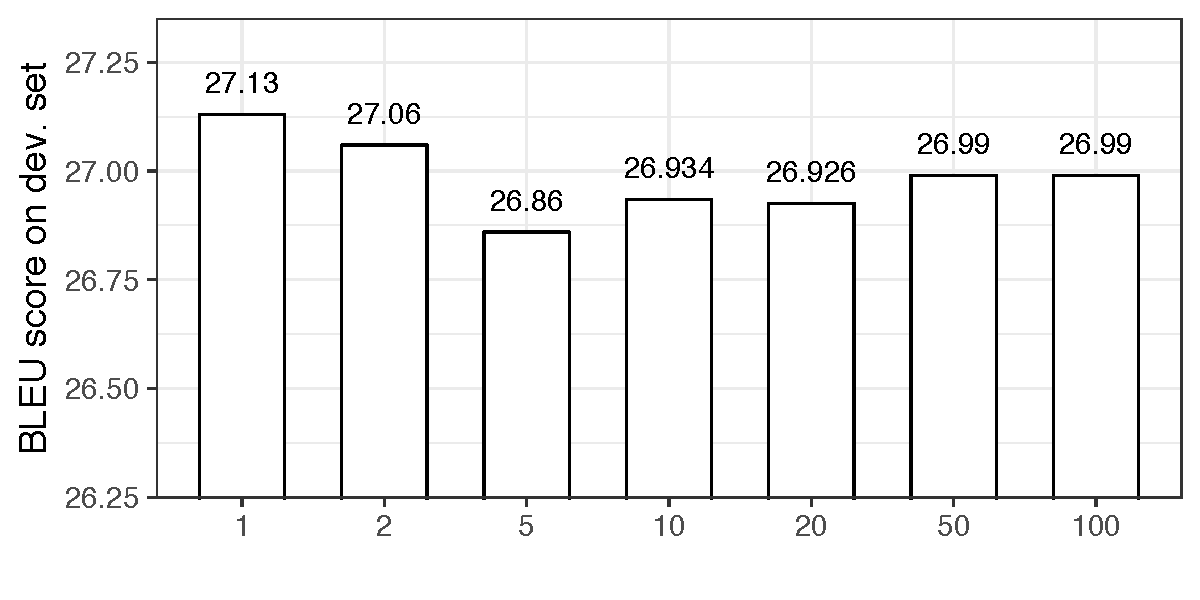
\includegraphics[width=0.7\columnwidth]{distill/approx}
	\caption{The effect of using different $K$s when approximating
		distillation loss with $K$-most probable actions in the machine translation experiments.}\label{fig:distill:approx}
\end{figure}

本文在一个IWSLT2014德-英机器翻译数据集上进行实验。
IWSLT2014德-英机器翻译数据集包含15.3万句训练数据,
7千句开发集数据,以及7千句测试集数据。
本文按照文献\inlinecite{DBLP:journals/corr/RanzatoCAZ15}
建议的方法对数据进行预处理,
并使用一个包含3万德语词以及2.5万英语词的词表作为模型的词表。
本文参考文献\inlinecite{wiseman-rush:2016:EMNLP2016}
并使用含有256个隐层单元的LSTM作为编码器与解码器。
本文使用BLEU\cite{papineni-EtAl:2002:ACL}评价机器翻译的
性能。\footnote{We use {\tt multi-bleu.perl} to evaluate our model's performance}
与依存句法分析实验类似,
本文汇报10次不同初始化条件下机器翻译模型的平均准确率。

优化公式\ref{eq:distill:distill}需要枚举所有可能的动作。
在神经机器翻译的情景下,由于词表非常大,
这种枚举往往是非常耗时耗力的。
为了使这种枚举可计算,本文使用根据
集成模型得到的$K$个最可能动作作为
整个$q(a\mid s)$概率分布的一种近似,
即优化
$\sum_a q(a \mid s) \cdot \log p(a \mid s) \approx
\sum_k^K q(\hat{a}_k \mid s) \cdot \log p(\hat{a}_k \mid s)$学习目标。
其中$\hat{a}_k$,是第$k$可能的动作。
为了研究$K$的近似能力,本文将$\alpha$固定为1,
通过调整$K$观察模型蒸馏的效果。
图\ref{fig:distill:approx}显示了这一结果。
从图\ref{fig:distill:approx}可见,$K$的不同并未带来显著的模型差异。
故出于速度考虑,本文在后续实验中设定$K$为1。

\subsection{结果}[Results]\label{sec:distill:exp-res}

\subsubsection{基于转移的依存句法分析}[Transition-based Dependency Parsing]
\begin{table}[t]
	\centering
	\begin{tabular}{lc}
		\hline
		& LAS \\
		\hline
		Baseline & 90.83  \\
		Ensemble (20) & 92.73 \\
		Distill (reference, $\alpha$=1.0) & 91.99 \\
		Distill (exploration, $T$=1.0) & 92.00 \\
		Distill (both) & 92.14 \\
		\hdashline
		Ballesteros等人,2016\cite{ballesteros-EtAl:2016:EMNLP2016}  (dyn. oracle) & 91.42 \\
		Andor等人,2016\cite{andor-EtAl:2016:P16-1} (local, B=1) & 91.02 \\
		\hdashline
		Buckman等人,2016\cite{buckman-ballesteros-dyer:2016:EMNLP2016} (local, B=8) & 91.19 \\
		Andor等人,2016\cite{andor-EtAl:2016:P16-1} (local, B=32) & 91.70 \\
		Andor等人,2016\cite{andor-EtAl:2016:P16-1} (global, B=32) & 92.79 \\
		Dozat与Manning,2016\cite{DBLP:journals/corr/DozatM16} & 94.08 \\
		Kuncoro等人,2016\cite{kuncoro-16} & 92.06 \\
		Kuncoro等人,2017\cite{kuncoro-17} & 94.60 \\
		\hline
	\end{tabular}
	\caption{The dependency parsing results. 
		Significance test \cite{NILSSON08.52} shows the improvement of our \textit{Distill (both)} over \textit{Baseline}
		is statistically significant with $p<0.01$.}\label{tbl:distill:parse-res}
\end{table}

表\ref{tbl:distill:parse-res}显示了PTB数据集上的实验结果。
这一结果显示集成模型高于基线模型1.90。
在将$\alpha$设置为1时,模型取得了最佳的开发集结果。
而此时测试集的准确率为91.99。

本文也研究了温度对于从探索状态中蒸馏的模型的影响。
图\ref{fig:distill:temperature}显示了这一结果。
根据表\ref{fig:distill:temperature},
在采样时使用尖锐的分布总体上取得了更好的开发集性能。
从探索状态蒸馏与从参考状态中蒸馏获得的模型的性能基本相当。
将两者结合进一步提高了准确率(带标签的依存关系准确率达到92.14)。

本文也在表\ref{tbl:distill:parse-res}中
将本文提出的模型与其他依存句法分析器进行了对比。
表\ref{tbl:distill:parse-res}的第二组显示了前人工作中
基于贪心解码的依存句法分析器的性能。
文献\inlinecite{andor-EtAl:2016:P16-1}
使用了与本文不同的状态表示方法,
同时分别研究了贪心解码与柱搜索(beam-search)的效果。
文献\inlinecite{ballesteros-EtAl:2016:EMNLP2016}
研究了使用动态参考策略(dynamic oracle)训练贪心解码的句法分析器
的问题。
本文提出的基于知识蒸馏的句法分析器的表现
好于这些基于贪心解码的句法分析器。
表\ref{tbl:distill:parse-res}显示了
其他依存句法分析算法的效果。
这些算法包括:在基于转移的句法分析中
使用柱搜索\cite{buckman-ballesteros-dyer:2016:EMNLP2016,andor-EtAl:2016:P16-1},
使用全局优化目标训练基于转移的依存句法分析\cite{andor-EtAl:2016:P16-1},
基于图的依存句法分析\cite{DBLP:journals/corr/DozatM16},
将基于图的依存句法分析器蒸馏到基于转移的依存句法分析器\cite{kuncoro-16},
以及将短语结构句法的结果通过规则转化为依存句法\cite{kuncoro-17}。
本文提出的基于知识蒸馏的方法由于这些基于转移的算法,
但相较其他算法仍有差距。
这类差距主要是由对问题的建模方式的不同导致的。

\subsubsection{神经机器翻译}[Neural Machine Translation]

\begin{table}[t]
	\centering
	\begin{tabular}{lc}
		\hline
		& BLEU \\
		\hline
		Baseline & 22.79 \\
		Ensemble (10) & 26.26 \\
		Distill (reference, $\alpha$=0.8) & 24.76 \\
		Distill (exploration, $T$=0.1) & 24.64 \\
		Distill (both) & 25.44 \\
		\hdashline
		MIXER & 20.73 \\
		BSO (local, B=1) & 22.53 \\
		BSO (global, B=1) & 23.83 \\
		\hline
	\end{tabular}
	\caption{The machine translation results.
		MIXER denotes that of \citet{DBLP:journals/corr/RanzatoCAZ15},
		BSO  denotes that of \citet{wiseman-rush:2016:EMNLP2016}.
		Significance test \cite{koehn:2004:EMNLP} shows the improvement of our \textit{Distill (both)} over \textit{Baseline}
		is statistically significant with $p<0.01$.
	}\label{tbl:distill:nmt-res}
\end{table}

\begin{figure}[t]
	\centering
	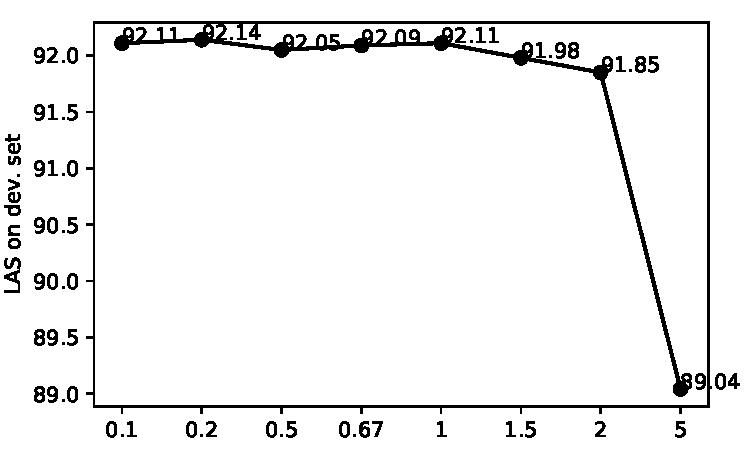
\includegraphics[width=0.7\columnwidth]{distill/temperature}
	\caption{The effect of $T$ on PTB (above)
		and IWSLT 2014 (below) development set.
	}\label{fig:distill:temperature}
\end{figure}

表\ref{tbl:distill:nmt-res}显示了IWSLT 2014数据集的机器翻译结果。
与PTB的结果类似的是,对10个模型进行集成的效果超过
基线系统3.47个BLEU值。
从参考状态中进行知识蒸馏能够获得BLEU值为24.76的单模型。


与基于转移的句法分析实验类似的是,
在采样过程中尖锐的分布带来的模型的效果更好,
然而,根据图\ref{fig:distill:temperature},
在$T\le0.2$的情况下,$T$的不同导致的差异并不明显。
在后续实验中,本文根据开发集结果设定$T=0.1$。
表\ref{tbl:distill:nmt-res}显示从探索状态中进行知识蒸馏的
模型获得24.64的准确率。
这一准确率相机从参考状态中蒸馏有微小的差异。
但将从参考中蒸馏和从探索中蒸馏进一步大幅度提高了准确率,
并且获得了25.44的BLEU值。

本文也将本文的模型与前人工作进行对比:
对比的系统包括基于强化学习的机器翻译\cite{DBLP:journals/corr/RanzatoCAZ15},
以及在翻译器学习过程中加入柱搜索\cite{wiseman-rush:2016:EMNLP2016}。
对比显示本文提出的模型取得了最优的结果。

上述句法分析与机器翻译实验
表明仅从探索状态中进行知识蒸馏是可行的。
同时将从参考状态中蒸馏与从探索状态中蒸馏进行结合可以进一步提高模型
性能,并取得超越其他贪心搜索模型的性能。

%\paragraph{Speed Comparison}
%
%\begin{table}
%	\centering
%	\begin{tabular}{rrcc}
%		\hline
%		model & beam & BLEU & speed \\
%		Baseline & 1 & & \\
%		& 5 & & \\
%		& 10 & & \\
%		\hline
%		Distill both & & & \\
%		\hline
%	\end{tabular}
%\caption{Speed comparison.}
%\end{table}
%
%Beam search generally improves search-based structured predictor's perform
%according to previous literals \cite{buckman-ballesteros-dyer:2016:EMNLP2016,wiseman-rush:2016:EMNLP2016}.
%We run a beam-search decoding on the baseline model.

\subsection{分析}[Analysis]\label{sec:analysis}

根据第\ref{sec:distill:exp-res}节的结果,
使用集成模型显著提高了依存句法分析以及神经机器翻译的性能够。
然而,类似``为什么集成模型如此有效?
能不能放弃传统对数似然学习目标,完全从知识蒸馏学习目标中学习?
以及从知识蒸馏中学习是不是稳定的?''一类的问题并么有得到很好的回答。
在这一节中,
本文首先研究集成模型在``错误状态''上的表现
证明其具有更好的泛化能力。
然后,本文通过研究公式\ref{eq:distill:distill}中的$a$的作用
经验性地证明了完全从知识蒸馏中学习的可行性。
最后,本文通过分析表明知识蒸馏可以带来更稳定的模型学习。

\subsubsection{模型集成对于``错误状态''的作用}[Ensemble on ``Problematic'' States]\label{sec:distill:ens-on-states}
\begin{table}[t]
	\centering
	\begin{tabular}{l  c c}
		\hline
		& optimal-yet-ambiguous & non-optimal \\
		\hline
		Baseline & 68.59 & 89.59\\
		Ensemble & 74.19 & 90.90 \\
		Distill (both) & 81.15 & 91.38 \\
		\hline
		%\hline
	\end{tabular}
	\caption{The ranking performance of parsers' 
		output distributions evaluated in MAP on
		``problematic'' states.}\label{tbl:state-ana}
\end{table}
As mentioned in previous sections, ``problematic'' states
which is either ambiguous or non-optimal harm structured prediciton's 
performance.
Ensemble shows to improve the performance in Section \ref{sec:exp-res}, 
which indicates it does better on these states.
To empirically testify this, we use dependency parsing as a testbed
and study the ensemble's output distribution
using the dynamic oracle.

The dynamic oracle  \cite{goldberg-nivre:2012:PAPERS,TACL302} 
can be used to efficiently determine, given any state $s$, which
transition action leads to the best achievable parse from $s$; 
if some errors may have already made, what is the best the parser can do,
going forward?  This allows us to analyze the accuracy of each
parser's individual decisions, in the ``problematic'' states.
In this paper, we evaluate the output distributions of the
baseline and ensemble parser against
the {\it reference actions} suggested by the dynamic oracle.
Since dynamic oracle yields more than one reference actions
due to ambiguities and previous mistakes and the output distribution
can be treated as their scoring, we evaluate them
as a ranking problem. Intuitively, when multiple reference actions exist,
a good parser should push probability mass to these actions.
We draw problematic states by sampling from our baseline parser.
The comparison in Table \ref{tbl:state-ana} shows
that the ensemble model significantly outperforms the baseline on ambiguous
and non-optimal states.
This observation indicates the ensemble's output distribution is more
``informative'', thus generalizes well on problematic states and achieves
better performance.
We also observe that the distillation model perform better than both the baseline and ensemble.
We attribute this to the fact that the distillation model is learned from exploration.
\subsubsection{Effect of $\alpha$}
\begin{figure}[t]
	\centering
	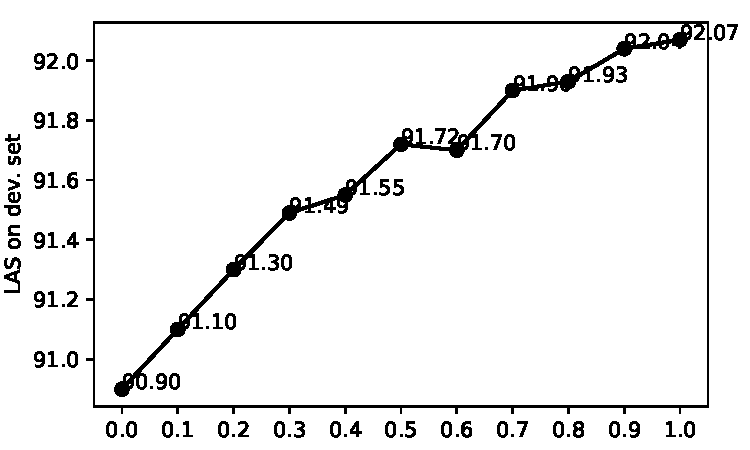
\includegraphics[width=0.7\columnwidth]{distill/alpha}
	\caption{The effect of $\alpha$ on PTB (above)
		and IWSLT 2014 (below) development set.
	}\label{fig:alpha}
\end{figure}

Over our distillation from reference model, we study the effect of $\alpha$ in Equation \ref{eq:distill}.
We vary $\alpha$ from 0 to 1 by a step of 0.1 in both the transition-based dependency parsing
and neural machine translation experiments
and plot the model's performance on development sets in Figure \ref{fig:alpha}.
Similar trends are witnessed in both these two experiments that
model that's configured with larger $\alpha$ generally performs better than that with
smaller $\alpha$.
For the dependency parsing problem, the best development performance is achieved
when we set $\alpha=1$, and for the machine translation, the best $\alpha$ is 0.8.
There is only 0.2 point of difference between the best $\alpha$ model
and the one with $\alpha$ equals to 1.
Such observation indicates that
when distilling from the reference policy paying more attention
to the distillation loss rather than the NLL is more beneficial.
It also indicates that fully learning from 
the distillation loss outputted by the ensemble is reasonable because models configured with
$\alpha=1$ generally achieves good performance.

%
%\subsubsection{Effect of Annealing}
%
%\begin{figure}[t]
%	\includegraphics[width=1\columnwidth]{graphics/anneal}
%	\caption{The effect of temperature.}\label{fig:anneal}
%\end{figure}
%
%The effect of annealing is shown in Figure \ref{fig:anneal}. This figure shows some
%differences between two tasks, which for dependency parsing, sharpening the distribution
%(with $\alpha>1$) generally performs better while for the machine translation, flattening
%the distribution is more helpful.
%The soft target of dependency parsing is more sharp than that of the machine translation.
%It's reasonable because the translation problems encounters more ambiguities.
%


\subsubsection{Learning Stability}
\begin{figure}[t]
	\centering
	\subfigure{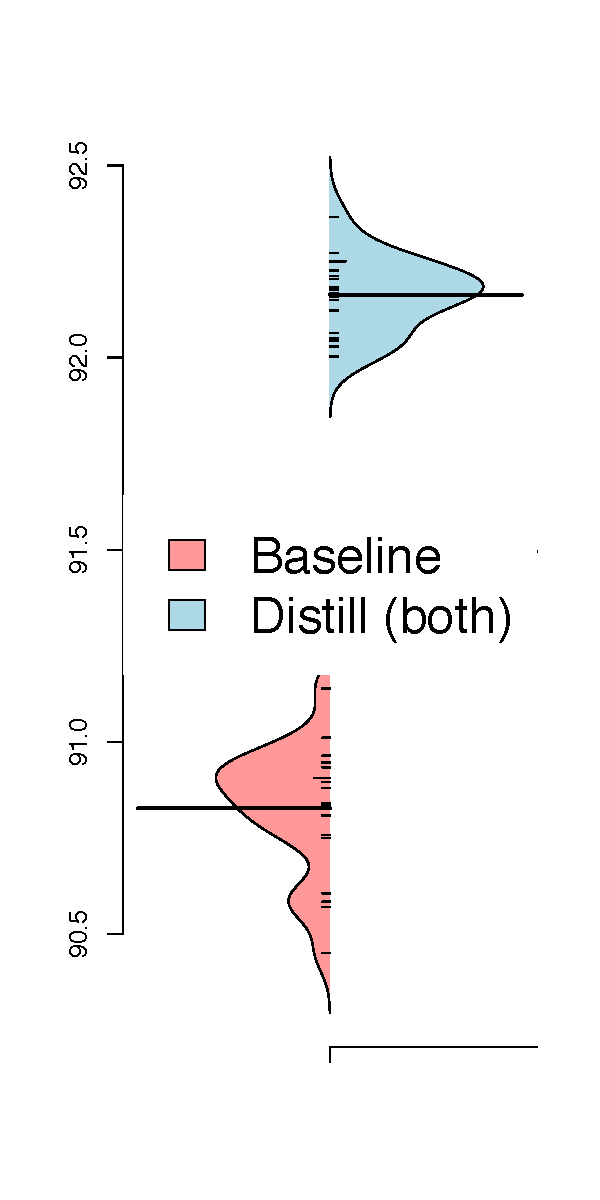
\includegraphics[width=0.4\columnwidth, trim={0, 1cm, 0, 1.5cm}, clip]{distill/stability_par_bean}}
	\subfigure{\includegraphics[width=0.4\columnwidth, trim={0, 1cm, 0, 1.5cm}, clip]{distill/stability_nmt_bean}}
	\caption{The distributions of scores for the baseline model and
		our {\it distillation from both} on PTB test (left) and IWSLT 2014 test (right)
		on differently-seeded runs.
	}\label{fig:stable}
\end{figure}

\begin{table}[t]
	\centering
	\begin{tabular}{rcccc}
		\hline
		system & seeds & min & max & $\sigma$ \\
		\hline
		\multicolumn{2}{r}{\it PTB test} & & & \\
		Baseline & 20 & 90.45 & 91.14 & 0.17 \\
		Distill (both) & 20 & 92.00 & 92.37 & 0.09 \\
		\hline
		\hline
		\multicolumn{2}{r}{\it IWSLT 2014 test} & & & \\
		Baseline & 10 & 21.63 & 23.67 & 0.55 \\
		Distill (both) & 10 & 24.22 & 25.65 & 0.12 \\
		\hline
	\end{tabular}
	\caption{The minimal, maximum, and standard derivation values
		on differently-seeded runs.}\label{tbl:stable}
\end{table}
Besides the improved performance,
knowledge distillation also leads to more stable learning.
The performance score distributions of differently-seed runs are depicted as
violin plot in Figure \ref{fig:stable}. Table \ref{tbl:stable}
also reveals the smaller standard derivations are achieved by
our distillation methods. As \citet{DBLP:journals/corr/KeskarMNST16} pointed out that
the generalization gap is not due to {\it overfit}, but due to
the network converge to {\it sharp minimizer} which generalizes worse,
we attribute the more stable training from our distillation model
as the distillation loss presents less {\it sharp minimizers}.

\section{相关工作}[Related Work]

Several works have been proposed to applying knowledge distillation
to NLP problems. \citet{kim-rush:2016:EMNLP2016} presented
a distillation model which focus on distilling the structured loss
from a large model into a small one which works on sequence-level.
In contrast to their work, we pay more attention to action-level distillation
and propose to do better action-level distillation by both from
reference and exploration.

\citet{DBLP:journals/corr/FreitagAS17} used an ensemble of 6-translators
to generate training reference.
Exploration was tried in their work with beam-search.
We differ their work by training the single model to match
the distribution of the ensemble.

Using ensemble in exploration was also studied in reinforcement learning
community \cite{NIPS2016_6501}.
In addition to distilling the ensemble on the labeled training data,
a line of semi-supervised learning works show that
it's effective to transfer knowledge of cumbersome model
into a simple one on the unlabeled data \cite{liang:icml08,li-zhang-chen:2014:P14-1}.
Their extensions to knowledge distillation call for further study.

\citet{kuncoro-16} proposed to compile the knowledge from
an ensemble of 20 transition-based parsers
into a voting and distill the knowledge
by introducing the voting results as a regularizer
in learning a graph-based parser.
Different from their work, we directly do the distillation on
the classifier of the transition-based parser.

Besides the attempts for directly using the  knowledge distillation technique,
\citet{stahlberg-byrne:2017:EMNLP2017} propose to first 
build the ensemble of several machine translators into one network by unfolding
and then use SVD to shrink its parameters, which can be treated as another kind of knowledge distillation.

\section{结论}[Conclusion]
In this paper, we study knowledge distillation for search-based structured prediction
and propose to distill an ensemble into a single model both from reference and exploration states.
Experiments on transition-based dependency parsing and machine translation
show that our distillation method significantly improves the single model's performance.
Comparison analysis gives empirically guarantee for our distillation method.
